Building on the extensive prior work that has led to a better understanding of
atomic-level anisotropy and its effect(s) on intermolecular interactions, we
now outline a methodology whereby atomic-level anisotropy can be incorporated
into standard force fields amenable to large-scale molecular
simulation. 
%% Before continuing, we must note that, especially given the diversity of prior approaches
%% used to treat atomic-level anisotropy, there is likely no one correct answer
%% as to how force fields should be extended to move beyond the sum-of-spheres
%% approximation. Indeed, we do not wish to provide the reader with the false
%% impression that our ansatz is the best, or only, way to model anisotropy.
%% Rather, 
In particular, we aim to present a general methodology that optimally incorporates
atomically-anisotropic effects given the following 
goals for ab initio force field development:

%TODO: Find a good place to include a discussion of ab-inito vs. empirical
%force field development

\begin{enumerate}
\item \textbf{Chemical accuracy with respect to ab initio benchmarks:} For systems that can be directly parameterized against
high quality ab initio PES, the force field should exhibit chemical
accuracy (average errors smaller than 1\kjmolold)
with respect to the ab initio benchmark; furthermore, any errors in the force
field should be random rather than systematic
%% \item \textbf{Chemical accuracy with respect to experiment:} Force fields for a given
%% compound should achieve chemical accuracy with respect to experimental
%% properties across all known phases (solid, liquid, supercritical, etc.) 
\item \textbf{Transferability across chemical environments:} Given force fields for two different pure systems, we
should be able to accurately calculate (via simple
combination rules and without additional
parameterization) the PES of any system that
is a mixture of the pure systems
%% \item \textbf{Universality:} There should be one universally-applicable (and
%% ideally automatable) methodology for force field
%% development that allows us to model (without over-reliance on chemical intuition or ad-hoc
%% inclusion of molecule-specific terms, parameters, or interaction sites) all
%% manner of intermolecular interactions; in other words, the same functinal
%% forms and parameterization scheme should be equally applicable to descriptions
%% of lone pairs, $\pi$ electrons, $\sigma$ holes, etc.
%% \item \textbf{Robustness:} The chosen force field development methodology should not be
%% overly sensitive to the details of parameterization, and the chosen
%% parameterization scheme should not result in either under- or over-fitting of
%% the potential
\item \textbf{Simplicity:} The force field should be restricted to functional forms
that are already compatible with, or could be easily implemented in, common
molecular simulation packages
\item \textbf{Computational tractability:} The force field should be of minimal computational cost
relative to existing polarizable multipolar force fields\cite{Shi2013}
\end{enumerate}

Given these goals, we now outline a detailed methodology for incorporating
atomic-level anisotropy into each component (electrostatic,
exchange-repulsion, induction, and dispersion) of intermolecular interactions,
beginning with a new model for
short-range overlap effects and concluding with some new and/or revised
theories for treating long-range interactions.

\begin{subsection}{Anisotropic Models for Short-Range Interactions}

% \begin{subsubsection}{A Note on Coordinate Systems}
% \end{subsubsection}

\begin{subsubsection}{Exchange-Repulsion}
\label{sec:exchange_theory}

We begin by considering the exchange-repulsion, $\erep_{ij}$ that arises from the overlap of
electron densities from two non-spherical atoms-in-molecules, $i$ and $j$. Here and
throughout, we closely follow the notation and theory used by
\citeauthor{stone2013theory}.\cite{stone2013theory}
Without loss of
generality, we can express the exchange repulsion between these two atoms as a
function of their interatomic distance, $r_{ij}$, and relative
orientation, $\Omega_{ij}$. Furthermore, we can mathematically describe this relative
orientation by assigning local coordinate axes to each $i$ and $j$, such that
the exchange energy is given by
%
\begin{align}
\label{eq:general_anisotropic_repulsion}
\erep_{ij}(r_{ij},\Omega_{ij}) \equiv
\erep_{ij}(r_{ij},\theta_i,\phi_i,\theta_j,\phi_j),
\end{align}
%
where $\theta_i$ and $\phi_i$ are the polar coordinates, expressed in the local
coordinate system of atom $i$, that describe the position of atom $j$.
Correspondingly, $\theta_j$ and $\phi_j$ define the position of $i$ in terms
of the local coordinate system of $j$. In principle the choice of these local coordinate
frames is arbitrary. However, for the models introduced below,
parameterization can be dramatically simplified by taking advantage of the
local symmetry of an atom in its molecular environment and aligning the local
coordinate frame with the principal axis of this local
symmetry.\cite{stone2013theory} Some examples of these local axes are shown in
\cref{fig:local_axis}.

          \begin{figure}
          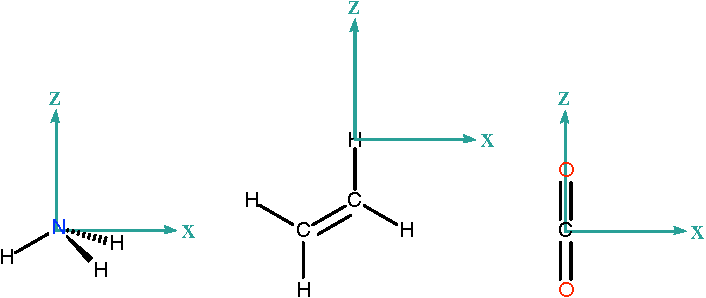
\includegraphics[width=0.9\textwidth]{anisotropic/figures/local_coords-crop.pdf}  
          \caption{Local axis system, shown for select atoms in molecules.}
          \label{fig:local_axis}
          \end{figure}

We next make an ansatz that \cref{eq:general_anisotropic_repulsion} is
separable into radial- and angular-dependent contributions,
%
\begin{align}
\label{eq:separable_anisotropic_repulsion}
%\erep_{ij}(r_{ij},\theta_i,\phi_i,\theta_j,\phi_j) \approx f(r_{ij})g(\theta_i,\phi_i,\theta_j,\phi_j),
\erep_{ij}(r_{ij},\theta_i,\phi_i,\theta_j,\phi_j) \approx 
\vrep_{ij}(r_{ij},\theta_i,\phi_i,\theta_j,\phi_j) = \fij \gij
\end{align}
%
thus subdividing the problem of finding a general functional form for $\erep_{ij}$ into
two more tractable tasks. First, we must find an ideal sum-of-spheres model to
describe the radial (isotropic) dependence of the force field, and second, we must find
a way to model the orientation dependence as a multiplicative
pre-factor to \fij.

% TODO: Include a discussion of additional forms for \fij that might serve as
% good functional forms upon which gij can be added?
Given that the only requirement for \fij is that it be isotropic, how should a
suitable model for \fij be chosen?
Indeed, all standard isotropic force fields are of this general form, and thus
might serve as a suitable starting point for anisotropic force field development.
For reasons discussed below, in this Chapter we employ 
a simple and accurate model (\isaffold) from \cref{ch:isaff} for \fij. This
model can be
derived from first-principles by approximating $\erep_{ij}$ as proportional to
the overlap %, $S_{\rho}^{ij}$,
between spherically-symmetric atom-in-molecule (AIM) electron densities, each with density
\begin{align}
\rho_i(r) = D_i \exp^{-B_i r},
\end{align}
where $D_i$ and $B_i$ are both atom type-specific constants that can be parameterized from
molecular electron densities and that represent, respectively,
the shape and hardness of the AIM density. Using this approximation to the
overlap model,
\cite{Kim1981,Nyeland1986,Ihm1990,Stone2007,Wheatley1990,Mitchell2000,Soderhjelm2006,Day2003}
the exchange energy between two atoms is then modeled by
%
\begin{align}
\begin{split}
\label{eq:fij}
\erep_{ij} \approx \vrep_{ij} &\propto S_{\rho}^{ij} \\
&\approx \Aex{ij} \left( \frac{ (\B\R)^2}{3} + \B\R + 1 \right) \exp(-\B\R) 
\end{split}
\intertext{with combining rules} 
\begin{split}
\label{eq:aij}
\Aex{ij} 
&\equiv \Aex{i}\Aex{j},\\
\B &\equiv \sqrt{B_iB_j}. \\
\end{split}
%
\end{align}
%
$S_{\rho}^{ij}$ is the electron density overlap between atoms and \A is
a fitted proportionality constant.

Here and throughout we use \cref{eq:fij}
as our
model for \fij. This choice is primarily justified in \cref{ch:isaff} by the
previously-demonstrated accuracy of the Slater-ISA formalism as compared to other
sum-of-spheres models for repulsion.\cite{VanVleet2016} 
Furthermore, and especially for simple test cases where one
might expect the sum-of-spheres approximation to hold (such as with argon, methane, or ethane), we have shown (see
\cref{ch:isaff}) that the \isaffold
correctly models intermolecular potential energy surfaces for a sizable library of intermolecular
interactions over the asymptotic, attractive, and repulsive regions of
the PES.

In addition to this empirical motivation for using the Slater-ISA formalism,
there are good theoretical grounds to utilize it as a model for \fij.
Specifically, the AIM densities used to parameterize \isaffold are
partitioned using an iterated stockholder atoms (ISA) procedure,
and the resulting density profiles are guaranteed to be maximally spherical.
\cite{Misquitta2014,Lillestolen2008,Lillestolen2009}
%DISCUSS: Alston, to what extent is this true? That is, are the BS-ISA
%densities algorithmically guaranteed to converge to maximally-spherical
%shapes, or does this just empirically seem to be true in practice?
This condition of `maximum sphericity' has two consequences. First, it
suggests that the resulting \isaffold should be an optimal, or nearly optimal,
isotropic atom-atom model. In other words, there is good reason to hope that
our model for \fij completely accounts for
the radial dependence of the potential, and consequently that models for \gij
will truly represent the orientation dependence rather than simply over-fitting
residual errors from the radial functional form, thus retaining high
transferability. 
Second, and relatedly,  having
maximally-spherical ISA densities suggests that anisotropic effects should be a
minimal perturbation to the PES. This means that, to a first-order
approximation, \gij is simply equal to 1. Furthermore, the non-spherical
components of the ISA densities should provide us
with guidance as to which atom types might require anisotropic treatment.

With the functional form for \fij determined, we now describe our
model for \gij. As motivated in \appendixref{sec:appendix}, and under
the ansatz of radial and angular separability,
an approximate, transferable, and orientation-dependent expression for \Aex{i} can be obtained
by expanding \Aex{i} in a
basis of 
renormalized spherical harmonics,
\begin{align}
\label{eq:sph_harm}
C_{lm}(\theta,\phi) = \sqrt{\frac{4\pi}{2l+1}}Y_{lm}(\theta,\phi).
\end{align}
thus yielding
%
\begin{align}
\label{eq:gij}
\begin{split}
\Aex{i}(\theta_i,\phi_i) &= 
\Aex{i,\text{iso}}\big(1 + \aniso{exch} \big), \\
\aniso{exch} &\equiv \sum\limits_{l>0,k} \aex  C_{lk}(\theta_i,\phi_i)
\end{split}
\end{align}
%
for \Aex{i} and subsequently
%
\begin{align}
\label{eq:vex}
\vrep_{ij} &= \Aex{ij}(\Omega_{ij})
        \left( \frac{ (\B\R)^2}{3} + \B\R + 1 \right) \exp(-\B\R)
\end{align}
with
\begin{align}
\Aex{ij}(\Omega_{ij}) &= \Aex{i}(\theta_i,\phi_i)\Aex{j}(\theta_j,\phi_j)
\end{align}
%
for the exchange-repulsion potential. Note that, with the exception of the
now orientation-dependent \Aex{i}, the atomically-anisotropic model in \cref{eq:vex} is identical to
our previously-defined isotropic model (\cref{eq:fij}). 

In terms of parameterization for our newly-developed anisotropic model, note
that the \aex are free parameters which must be fit to ab initio
data. 
Still, we and others have found the expansion in \cref{eq:gij} to be very quickly convergent,
\cite{Stone2007,Mitchell2001,Price2000,Stone1988,Day2003,Torheyden2006,Totton2010,Misquitta2016,Price2010a}
 especially given a proper choice of coordinate
system that eliminates many expansion terms via symmetry. In practice, only
symmetry-allowed terms up
to $l=2$ seem to be required for heteroatoms, carbons in multiple bonding
environments, and select hydrogens (see
equations in \cref{sec:results}), while many other atom types require no anisotropic
parameters whatsoever. Encouragingly,
isotropic atom types are easily modeled within
this formalism simply by setting $\aniso{} = 0$.

\end{subsubsection}
\begin{subsubsection}{Other Short-Range Effects}

As in \cref{ch:isaff},\cite{VanVleet2016} we have found that other short-range effects, namely charge
penetration and short-range induction, can be modeled as proportional to
exchange-repulsion. We take the same approach in the present Chapter, and
the functional form for these two short-range effects is given by
\cref{eq:vex}, with `exch' superscripts replaced by the appropriate short-range
energy term (see \cref{sec:methods}).
Additionally, for induction, the long-range polarization must be damped, and
for now this damping is modeled isotropically
as in the AMOEBA force field.\cite{Shi2013} 
%
Finally, to model short-range dispersion, we
take the same Tang-Toennies\cite{Tang1984,Tang1992} damping approach as in
\cref{ch:isaff}.\cite{VanVleet2016} Because the argument to the damping function is given by 
\[
x = -\frac{d}{dr}\left[\ln \vrep(r)\right] \ r,
\]
and because anisotropy only enters into the functional form as a
multiplicative pre-factor, our functional form for damping remains unchanged
compared to our previously-derived isotropic model.\cite{VanVleet2016}

\end{subsubsection}
\end{subsection}

\begin{subsection}{Anisotropic Models for Long-Range Interactions}

\begin{subsubsection}{Electrostatics}

Theories for including anisotropy in long-range electrostatics are well
established, and we refer the reader
elsewhere for complete details on the required formalisms for distributed multipole approaches.
\cite{stone2013theory,Stone2007}
In the present Chapter, 
\[
V^{\text{multipole}}_{ij} = \vmultipole
\]
with multipolar interaction tensor $T$ and parameterized moments $Q$ for all
multipole moments $tu$ up to (in the present Chapter) rank 2.

On the grounds of increased accuracy and ease of parameterization, here we have chosen 
to use a multipolar approach to describe the anisotropy of
long-range electrostatics,
However, for increased computational efficiency, off-site point charge models
\cite{Cardamone2014}
could also be utilized.

\end{subsubsection}
\begin{subsubsection}{Induction}

Just as with electrostatics, long-range induction should properly be described
by a distributed multipole expansion of interacting atomic
polarizabilities.\cite{Stone2007,Misquitta2016} Indeed, it has been shown
that inclusion of higher-order and/or anisotropic polarizabilities greatly
reduces errors in the two-body induction potential relative to commonly-used isotropic
dipole polarizability models.\cite{Misquitta2008b,Holt2008,Holt2010,Schmidt2015,Shi2013}
Because the model for the two-body induction also determines the many-body
polarization energy, the proper treatment of induced multipoles becomes especially
important in condensed phase simulation.\cite{stone2013theory,Schmidt2015,Shi2013}

Owing to the increased computational cost of these higher-order and anisotropic polarizability
models, and because such functional forms are (as of now, and to our
knowledge) not fully implemented in common molecular simulation packages, we
neglect
both higher-order and anisotropic contributions to the long-range induction in
the present Chapter. As
we shall show, however, errors in the induction potential limit the overall accuracy of
our force fields for extremely polar molecules (notably water), and
further improvements will likely require us to generate improved models for long-range induction. 

\end{subsubsection}
\begin{subsubsection}{Dispersion}

Past research\cite{stone2013theory} has motivated an anisotropic atom-atom model for dispersion 
of the form
%
% TODO: Check the limits on this equation
\begin{align}
\label{eq:stone_disp}
\vdisp_{ij} = - \sum\limits_{n=6} \frac{C_{ij,n}(\Omega_{ij})}{\R^n}
\end{align}
%
Note that, in this equation, both odd and even powers of $n$ are allowed in the
dispersion expansion.
In order to make this model both computationally efficient and maximally compatible with our previous isotropic
model for dispersion, 
%% and in a manner analogous to our treatment of
%% short-range overlap effects, 
we choose (as an ansatz) to model the dispersion anisotropy as an
orientation-dependent prefactor that effects all isotropic $C_6 - C_{12}$ dispersion
coefficients equally:
%
\begin{align}
\label{eq:mastiff_disp}
\vdisp_{ij} &= - \Adisp{i}\Adisp{j}\sum\limits_{n=3}^{6} \frac{C_{ij,2n}}{\R^{2n}} 
\intertext{with}
\label{eq:mastiff_disp2}
\Adisp{i} &= 1 + \aniso{disp}
\end{align}
%
and \aniso{disp} as in \cref{eq:gij}.
%% Because $C_{00}(\theta,\phi) = 1$, the anisotropy expansion proposed above has
%% no effect on the average magnitude of the various dispersion coefficients.
Once again, \cref{eq:mastiff_disp} reduces to the isotropic case by setting
$\aniso{disp} = 0$.
%
We must note that, though the functional form in \cref{eq:mastiff_disp} bears many similarities to
\cref{eq:stone_disp}, (unphysically) no odd powers of $r$ show
up in our proposed model for dispersion. Furthermore, 
the model utilizes the same anisotropic expansion for each dispersion
coefficient.
Nonetheless, we will show in \cref{sec:results}
that this model yields significant accuracy gains in the dispersion energy
with only minimal additional parameterization and model expense.

\end{subsubsection}


\end{subsection}
